
\documentclass[11pt]{article}

%\setlength\topmargin{-0.1in}
%\setlength\headheight{0in}
%\setlength\headsep{0in}
\setlength\textheight{8.5in}
\setlength\textwidth{6.5in}
\setlength\oddsidemargin{0in}
\setlength\evensidemargin{0in}
\setlength{\parindent}{0pt}
\usepackage{placeins}
%\usepackage{indentfirst}

\usepackage{amsmath}
\usepackage{graphicx}
\usepackage{listings}
\usepackage{rotating}
\usepackage{subcaption} 
\usepackage{booktabs}
\usepackage{tikz}
\usepackage{fancyhdr}
\usepackage{pdfpages}
\usepackage{hyperref}
\usepackage{longtable}
\usepackage[toc,page]{appendix}
%For The 2x2 Figure
\usepackage{subcaption}
\usepackage{mwe}
% To import matlab code
\usepackage{listings}
\usepackage{matlab-prettifier}
\usepackage[framed,numbered,autolinebreaks,useliterate]{mcode}
%Glossary
\usepackage[acronym,nonumberlist]{glossaries}
%\glsaddall %includes all acronymns
%Tables
\usepackage{booktabs}
\newcommand{\ra}[1]{\renewcommand{\arraystretch}{#1}}
%Nomenclature
\usepackage{nomencl}
\makenomenclature
\newif\iffirstglossary\firstglossarytrue
%% This removes the main title:
\renewcommand{\nomname}{}
%% this modifies item separation:
\setlength{\nomitemsep}{15pt}
%% this part defines the groups:
%----------------------------------------------
\usepackage{etoolbox}
\renewcommand\nomgroup[1]{%
  \item[\Large\bfseries
  \ifstrequal{#1}{N}{Nomenclature}{%
  \ifstrequal{#1}{A}{List of Abbreviations}{}}%
]\vspace{10pt}} % this is to add vertical space between the groups.
%----------------------------------------------



\pagestyle{fancy}
\usetikzlibrary{shapes,arrows}
\graphicspath{{Figures/}}
\newcommand{\tabitem}{~~\llap{\textbullet}~~}

\newcommand*{\MyIndent}{\hspace*{0.5cm}}%inerts tab in tables



 
\begin{document} 
\pagenumbering{gobble}

	\begin{titlepage}
	\thispagestyle{empty}
		\newcommand{\HRule}{\rule{\linewidth}{0.5mm}}	
		\center
		\LARGE 
		University of Bath\\
	 	Faculty of Engineering \& Design\\[1cm]	
		%textbf{\Large ME30313 Group Business & Design}\\
		\large
		Word count: 1584\\[0.5cm]
		{\large\today}\\[1cm]	
		\HRule\\[0.4cm]	
		{\LARGE \bfseries Systems Modelling \& Simulation Coursework 1}\\[0.3cm] 	
		\HRule\\[1cm]	
		\begin{minipage}{0.4\textwidth}
			\begin{flushleft}
				\large
				\textit{Supervisor}\\
				A. \textsc{Cookson}
			\end{flushleft}
		\end{minipage}
		~
		\begin{minipage}{0.4\textwidth}
			\begin{flushright}
				\large
				\textit{Assessor}\\
				
			\end{flushright}
		\end{minipage}\\[1.4cm]
		\large
		\textit{Author's Candidate Number}\\
		10838\\
		\vfill
		
\includegraphics[width=0.4\textwidth]{UOB_Logo.png}\\
		\vfill 
	\end{titlepage}

%%% ACRONYMS %%

%%END OF ACRONYMS %%%


\thispagestyle{empty}




\tableofcontents
\thispagestyle{empty}
\listoffigures


\nomenclature[A]{CAD}{Computer Aided Design}


%\printnomenclature


\clearpage
\pagenumbering{arabic}
%\setcounter{page}{1}
\section{Introduction}

This paper is based on solving the static diffusion-reaction equation given by equation \ref{eq:MAIN}.


\begin{equation}\label{eq:MAIN}
D \frac{\partial^2 c}{\partial x^2} + \lambda c + f = 0
\end{equation}

The weak form of this equation after integration by parts will be the starting point for derivations and is given by equation \ref{eq:MAINWEAK}.
\begin{equation} \label{eq:MAINWEAK}
\int D \frac{\partial c}{\partial x}  \frac{\partial v}{\partial x}  dx - \int \lambda cvdx  = \int vf dx + \left[vD\frac{\partial c}{\partial x} \right]
\end{equation}


\section{Part 1: Software Verification \& Analytical Testing}

\subsection{Question 1a}
\subsubsection{Derivation of Diffusion Element Matrix}

The 2-by-2 element matrix for a diffusion operator for an arbitrary element $e_{n}$ between the points $x_{0}$ $x_{1}$ shall be derived.  The derivation shall start from the weak form version of the static diffusion-reaction equation, after performing integration by parts, which is given by equation \ref{eq:MAINWEAK}.  To obtain the diffusion element matrix only the diffusion integral needs to be evaluated which will be done over the domain $x = 0$ to $x = 1$. The resulting integral to be evaluated is given by equation \ref{eq:weakformdiff}

\begin{equation} \label{eq:weakformdiff}
\int_0^1 D \frac{\partial c}{\partial x}  \frac{\partial v}{\partial x}  dx 
\end{equation}

The domain from $x = 0$ to $ x = 1$ can be split into $ne$ number of elements. This is shown pictorially by Figure \ref{fig:domain2elements} for the case $ne = 4$.

%Figure to show elements on a line
\begin{figure}[h!]
\centering
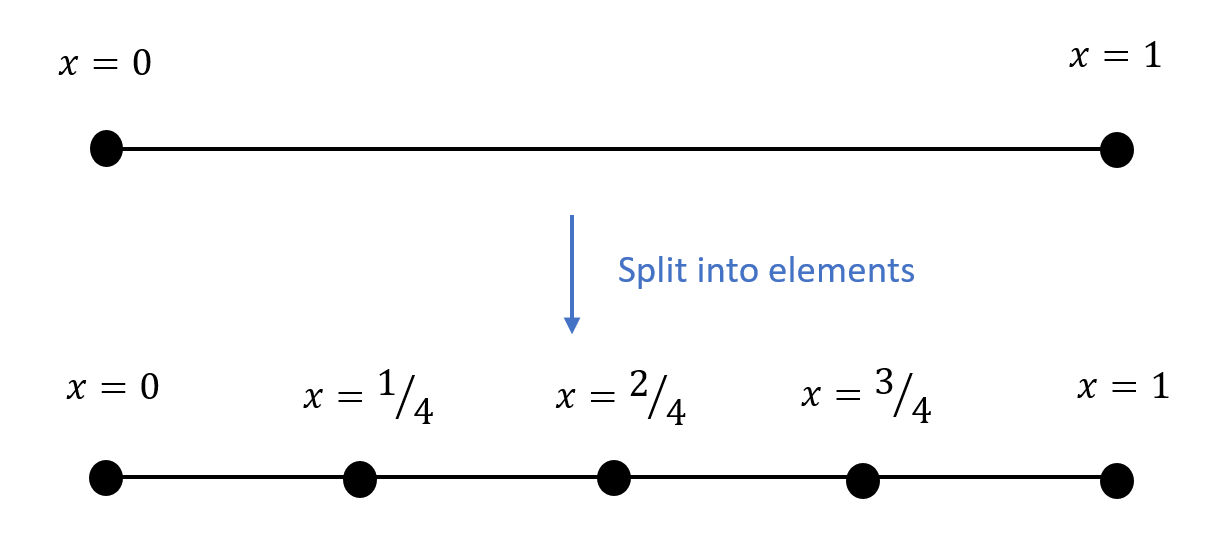
\includegraphics[width=0.75\textwidth]{SplitIntoElements.PNG}
\caption{Splitting Domain Into Equispaced Elements}\label{fig:domain2elements}
\end{figure}

Now the integral from $x = 0$ to $x = 1$ can be split into the sum of the integrals of the individual elements as demonstrated by equation \ref{eq:splitintegral} for the $ne = 4$ case.


%Splitting Intergral into elements
\begin{equation}
\label{eq:splitintegral}
\int_0^1 dx = \int_0^\frac{1}{4}  dx + \int_\frac{1}{4}^\frac{2}{4}  dx + \int_\frac{2}{4}^\frac{3}{4}  dx + \int_\frac{3}{4}^1  dx
\end{equation}

To solve the integrals the Galerkin formulation will be used were $c$ and $x$ are represented by linear Lagrange nodal functions as shown by equations \ref{eq:LagrangeC} and \ref{eq:LagrangeX}. As per the Galerkin assumption the test function $v$ is set equal to the basis function $\psi$ in order to minimise the residual error.




\begin{subequations}
\begin{equation}
\label{eq:LagrangeC}
c = c_{0}\psi_{0}(\zeta) + c_1\psi_{1}(\zeta) 
\end{equation}
\begin{equation}
\label{eq:LagrangeX}
x = x_{0}\psi_{0}(\zeta) + x_1\psi_{1}(\zeta)  
\end{equation}
\end{subequations}
\begin{equation}
\label{eq:LagrangeV}
v  = \psi_{0} , \psi_{1} 
\end{equation} 
where,
\begin{equation}
\label{eq:LagrangePSI}
\psi_{0} = \frac{1 - \zeta}{2} \ \ \ \ ,  \ \ \ \ \psi_{1} = \frac{1 + \zeta}{2} 
\end{equation}
and
\begin{equation}
\label{eq:LagrangeZeta}
\zeta   = 2 \left(\frac{x - x_0}{x_1 - x_0}\right) - 1 
\end{equation}


\hspace{10mm} for $x$ in that element between $x_0$ and $x_1$. \vspace{2mm}

The local element shall be mapped to a standard element using the Jacobian transform $J$, given by equation \ref{eq:Jacobian}, to map from the $x$ to the $\zeta$ coordinate system. The transform is shown pictorially in Figure \ref{fig:local2standard} for the second element of a four element equispaced mesh.


%Local element to standard element
\begin{equation} \label{eq:Jacobian}
J = \left \vert \frac{dx}{d\zeta}\right \vert
\end{equation}



%Figure to show elements mapping to standard
\begin{figure}[h!]
\centering
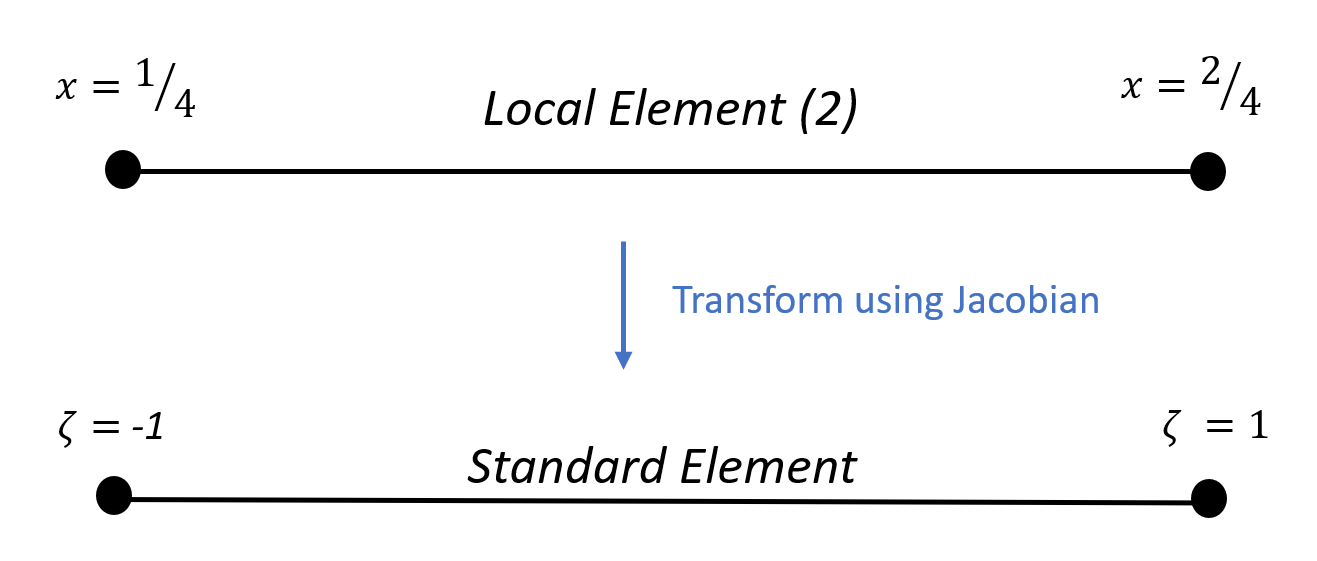
\includegraphics[width=0.75\textwidth]{Local2Standard.PNG}
\caption{Mapping to Standard Element}\label{fig:local2standard}
\end{figure}

The diffusion integral for a single element can now be mapped to the integral of a standard element using $dx = Jd\zeta$ which is a rearrangement of equation \ref{eq:Jacobian} and equation \ref{eq:LagrangeZeta} to transform the limits of integration. The result is given by equation \ref{eq:LHStransform}.

\begin{equation}
\label{eq:LHStransform}
\int_{x_0}^{x_{1}} D \frac{\partial c}{\partial x}  \frac{\partial v}{\partial x}  dx =  \int_{-1}^{1} D \frac{\partial c}{\partial x}  \frac{\partial v}{\partial x} J d\zeta
\end{equation}

It is necessary to evaluate the derivatives $\frac{\partial c}{\partial x}$ and $ \frac{\partial v}{\partial x}$ which can be obtain by applying the chain rule to the definitions of $c$ and $v$ given by equations \ref{eq:LagrangeC} and \ref{eq:LagrangeV}. The results are given by equations \ref{eq:LagrangeDC} and \ref{eq:LagrangeDV}.

\begin{align}\label{eq:LagrangeDC}
\frac{dc}{dx} &= c_{0}\frac{d\psi_{0}}{d\zeta}\frac{d\zeta}{dx} + c_1\frac{d\psi_{1}}{d\zeta}\frac{d\zeta}{dx}\\
 &= c_n\frac{d\psi_{n}}{d\zeta}\frac{d\zeta}{dx} \label{eq:LagrangeDC} \ \ \ \text{for} \ n =0,1 \nonumber
\end{align}
\begin{equation}
\label{eq:LagrangeDV} 
\frac{dv}{dx} = \frac{d\psi_{m}}{d\zeta}\frac{d\zeta}{dx} \ \ \ \text{for} \ m =0,1 
\end{equation}

The right hand side of equation \ref{eq:LHStransform} can now be rewritten as equation \ref{eq:LHStransform2}, recognising $c_n$ is independent of $x$ and therefore $\zeta$.
\begin{equation} \label{eq:LHStransform2}
 c_n\int_{-1}^{1} D \frac{d\psi_{n}}{d\zeta}\frac{d\zeta}{dx} \frac{d\psi_{m}}{d\zeta}\frac{d\zeta}{dx} J d\zeta
\end{equation}

Knowing that $\frac{d\zeta}{dx} = J^{-1}$ (for $x_1 > x_0$) from equation \ref{eq:Jacobian} and that for a given element $J$ is constant, equation \ref{eq:LHStransform} can be rewritten as equation \ref{eq:LHStransform3}.

\begin{equation} \label{eq:LHStransform3}
 c_nJ^{-1}\int_{-1}^{1} D \frac{d\psi_{n}}{d\zeta}\frac{d\psi_{m}}{d\zeta} d\zeta \ \ \ \ \text{for \ } n= 0,1 \ \text{\&}  \ m = 0,1
\end{equation}


Equation \ref{eq:LHStransform3} gives two equations which, when written in full, is clearly suitable for matrix representation.

\begin{subequations}
\label{eq:matrixform}
\begin{align}
&J^{-1} \left  [c_0 \int_{-1}^{1} D \frac{d\psi_{0}}{d\zeta} \frac{d\psi_{0}}{d \zeta} d \zeta + c_1 \int_{-1}^{1} D \frac{d\psi_{1}}{d\zeta} \frac{d\psi_{0}}{d\zeta}d\zeta ) \right ] \label{eq:row1} \\
&J^{-1} \left  [ c_0 \int_{-1}^{1} D \frac{d\psi_{1}}{d\zeta} \frac{d\psi_{0}}{d \zeta} d \zeta + c_1 \int_{-1}^{1} D \frac{d\psi_{1}}{d\zeta} \frac{d\psi_{1}}{d\zeta}d\zeta ) \right ] \label{eq:row2} 
\end{align}
\end{subequations}

The matrix representation is as follows where $I_{nm}$ represents the individual integrals in the above equations \ref{eq:row1} and \ref{eq:row2}. 

%%%	MATRIX Int_nm%%%%%
\begin{equation}
J^{-1}
\begin{bmatrix}

Int_{00} & Int_{01} \\
Int_{10} & Int_{11}
\end{bmatrix}
\begin{bmatrix}

c_{0} \\  c_{1} 
\end{bmatrix}
\end{equation}

%%Evaluate integrals%%%%%%%%%
Each $Int_{nm}$ term shall now be evaluated individually. In order to evaluate the integrals first the  derivatives of $\psi_0$ and $\psi_{1}$ with respect to $\zeta$ shall be calculated using the definition of the test function given by equation \ref{eq:LagrangePSI}. The results are given by equations 

\begin{subequations}
\label{eq:prematrix}
\begin{align}
\frac{d\psi_{0}}{d\zeta} &= \frac{d}{d\zeta}(\frac{1-\zeta}{2}) = -\frac{1}{2} \label{eq:psi0der}\\
\frac{d\psi_{1}}{d\zeta} &= \frac{d}{d\zeta}(\frac{1+\zeta}{2}) = \frac{1}{2} \label{eq:psi1der}
\end{align}
\end{subequations}
\\


\underline{$Int_{00}$} \\


\begin{equation}\label{eq:Int00}
\begin{split}
 Int_{00} &= \int_{-1}^{1} D \frac{d\psi_{0}}{d\zeta} \frac{d\psi_{0}}{d \zeta} d \zeta \\
&=  \int_{-1}^{1} D .( -\frac{1}{2}). (-\frac{1}{2}) d\zeta \\
& = \left[ \frac{D}{4} \zeta \right]_{-1}^{1} \\
& = \left[ (\frac{D}{4}.1) - (\frac{D}{4}.-1) \right] \\
& = \frac{D}{2}
\end{split}
\end{equation}

\underline{$Int_{01}$} \\


\begin{equation}\label{eq:Int01}
\begin{split}
 Int_{01} &= \int_{-1}^{1} D \frac{d\psi_{0}}{d\zeta} \frac{d\psi_{1}}{d \zeta} d \zeta \\
&=  \int_{-1}^{1} D .( -\frac{1}{2}). (\frac{1}{2}) d\zeta \\
& = \left[-\frac{D}{4} \zeta \right]_{-1}^{1} \\
& = \left[ (-\frac{D}{4}.1) - (-\frac{D}{4}.-1) \right] \\
& = -\frac{D}{2}
\end{split}
\end{equation}

\underline{$Int_{10}$} \\


\begin{equation}\label{eq:Int10}
\begin{split}
 Int_{01} &= \int_{-1}^{1} D \frac{d\psi_{1}}{d\zeta} \frac{d\psi_{0}}{d \zeta} d \zeta \\
&=  \int_{-1}^{1} D .( \frac{1}{2}). (-\frac{1}{2}) d\zeta \\
& = \left[-\frac{D}{4} \zeta \right]_{-1}^{1} \\
& = \left[ (-\frac{D}{4}.1) - (-\frac{D}{4}.-1) \right] \\
& = -\frac{D}{2}
\end{split}
\end{equation}


\clearpage

\underline{$Int_{11}$} \\


\begin{equation}\label{eq:Int11}
\begin{split}
 Int_{11} &= \int_{-1}^{1} D \frac{d\psi_{1}}{d\zeta} \frac{d\psi_{1}}{d \zeta} d \zeta \\
&=  \int_{-1}^{1} D .( \frac{1}{2}). (\frac{1}{2}) d\zeta \\
& = \left [\frac{D}{4} \zeta \right ]_{-1}^{1} \\
& = \left [ (\frac{D}{4}.1) - (\frac{D}{4}.-1) \right ] \\
& = \frac{D}{2}
\end{split}
\end{equation}

The local element matrix for the diffusion integral can now be assembled (not including the c term matrix). This is the form used in the code for LaplaceElemMatrix.m function available in Appendix \ref{ap:LaplaceElem}. Where J and D are scalars (we have assumed D to be constant).

%%%	Final MATRIX Int_nm%%%%%
\begin{equation} \label{eq:diffmatrix}
J^{-1}D
\begin{bmatrix}

0.5 & -0.5 \\
-0.5 & 0.5
\end{bmatrix}
\end{equation}

%%%%PASSING THE UNIT TEST Q1a%%%%%%%%%%%%

\subsubsection{Passes Unit Tests}

Figure \ref{fig:passTest1} shows the function LaplaceElemMatrix.m passes the unit tests defined in CourseworkOneUnitTest.m, available in Appendix \ref{ap:CW1}, with no errors.

%Screenshot pass unit test
\begin{figure}[h!]
	\centering
	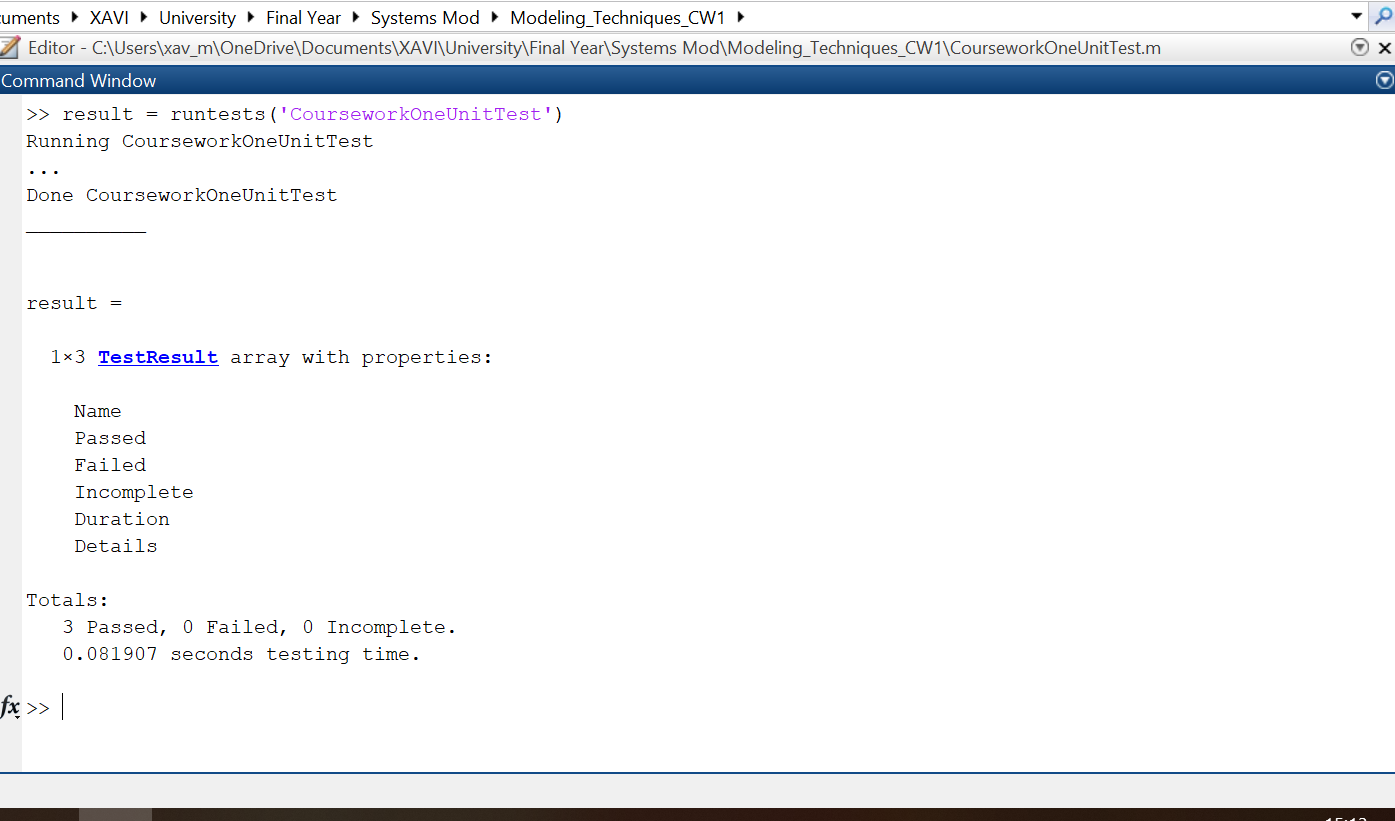
\includegraphics[width=0.75\textwidth]{CW1Test.PNG}
	\caption{Screenshot of LaplaceElemMatrix.m Function Passing Unit Tests}\label{fig:passTest1}
\end{figure}



\subsection{Question 1b}
\subsubsection{Derivation of Reaction Element Matrix}

The local reaction element matrix shall now be derived. This is found by evaluating the reaction integral, equation \ref{eq:reation1}, from the starting point for derivations equation \ref{eq:MAINWEAK}.

\begin{equation} \label{eq:reation1}
\int_{x_{0}}^{x_{1}} \lambda c v  dx
\end{equation}

As with the diffusion derivation the Jacobi is applied to map to the $\zeta$ domain. This gives equation \ref{eq:reactJ}.

\begin{equation}
\label{eq:reactJ}
\int_{-1}^1 \lambda c v J d\zeta
\end{equation}

The basis function for $c$ defined by equation \ref{eq:LagrangeC} and the Galerkin assumption for $v$ given by equation \ref{eq:LagrangeV} shall be used. Equation \ref{eq:reactJ} can then be written as set of two equations, similar to equations \ref{eq:row1} and \ref{eq:row2}. Assuming $\lambda$ to be independent of $x$ gives equations \ref{eq:reactrow1} and \ref{eq:reactrow1}. These equations can also be written in the form of a matrix as shown by equation \ref{eq:reactunsolvedmatrix}.

\begin{subequations}
\label{eq:reactsim}
\begin{align}
&J \lambda \left  [c_0 \int_{-1}^{1} \psi_{0} \psi_{0} d \zeta + c_1 \int_{-1}^{1} \psi_{1} \psi_{0} d\zeta ) \right ] \label{eq:reactrow1} \\
&J \lambda \left  [c_0 \int_{-1}^{1} \psi_{0} \psi_{1} d \zeta + c_1 \int_{-1}^{1} \psi_{1} \psi_{1} d\zeta ) \right ]  \label{eq:reactrow2} 
\end{align}
\end{subequations}



\begin{equation} \label{eq:reactunsolvedmatrix}
J \lambda
\begin{bmatrix}

Int_{00} & Int_{01} \\
Int_{10} & Int_{11}
\end{bmatrix}
\begin{bmatrix}

c_{0} \\  c_{1} 
\end{bmatrix}
\end{equation}
\\
The $Int_{nm}$ integrals shall be evaluated to derive the matrix. This requires substituting in the definitions of $\psi_0$ and $\psi_1$ given by equation \ref{eq:LagrangePSI}. \\

\underline{$Int_{00}$} \\
\begin{equation}\label{eq:Int00}
\begin{split}
 Int_{00} &= \int_{-1}^{1} \psi_{0}\psi_{0} \ d \zeta \\
&=  \int_{-1}^{1}  \Big ( \frac{1-\zeta}{2} \Big )^2 d\zeta \\
& = \left[ \frac{1}{3} \Big ( \frac{1-\zeta}{2} \Big )^3 (-2) \right]_{-1}^{1} \\
& = \frac{2}{3}
\end{split}
\end{equation} \\

\underline{$Int_{01} = Int_{10}$} \\

\begin{equation}\label{eq:Int01}
\begin{split}
 Int_{00} &= \int_{-1}^{1} \psi_{0}\psi_{1} \ d \zeta \\
&=  \int_{-1}^{1}  \Big ( \frac{1-\zeta}{2} \Big )  \Big ( \frac{1+\zeta}{2} \Big )d\zeta \\
& = \left[ \frac{\zeta}{4} - \frac{\zeta^3}{12}\right]_{-1}^{1} \\
& = \left[ \frac{1}{6} -  \Big (-\frac{1}{4} + \frac{1}{12} \Big )\right]_{-1}^{1} \\
& = \frac{1}{3}
\end{split}
\end{equation} \\

\underline{$Int_{11}$} \\
\begin{equation}\label{eq:Int00}
\begin{split}
 Int_{00} &= \int_{-1}^{1} \psi_{1}\psi_{1} \ d \zeta \\
&=  \int_{-1}^{1}  \Big ( \frac{1+\zeta}{2} \Big )^2 d\zeta \\
& = \left[ \frac{1}{3} \Big ( \frac{1+\zeta}{2}\Big)^3 . 2 \right]_{-1}^{1} \\
& = \frac{2}{3}
\end{split}
\end{equation} \\

Putting the results of the integrals into the matrix from equation \ref{eq:reactunsolvedmatrix} gives the result shown by equation \ref{eq:reactmatrix}. This result is used by the LinearReactionElemMatrix.m function available in Appendix \ref{ap:React}.\\


%%%	Reaction Matrix%%%%%
\begin{equation} \label{eq:reactmatrix}
J\lambda
\begin{bmatrix}

\frac{2}{3} & \frac{1}{3}  \\[1ex]
 \frac{1}{3}  & \frac{2}{3}
\end{bmatrix}
\end{equation}\\

 As per equation \ref{eq:MAINWEAK} this result needs to be subtracted from the local diffusion element matrix result given by equation \ref{eq:diffmatrix} in order to get the overall local element matrix which can then assemble into an global matrix. The global matrix is assembled in this way in the function StaticReactDiffSolver.m available in Appendix \ref{ap:SDRS}

%%%UNIT TEST FOR 1BBBBBB \\\\\\\\\\\\\\\\\\\\\\\\\\\%%%%%%%%%%%%
\subsubsection{Linear Reaction Element Matrix Unit Test}

A test script with four unit tests was made to check that the Linear Reaction Element Matrix function was working correctly. The tests were as follows\\
\begin{enumerate}
\item{Check outputted matrix is symmetrical}
\item{Two outputs for two elements in an equispaced mesh are the same }
\item{Check against known solution from (from tutorial 3 q2c solution).}
\item{Element 11 is double the value of element 21 for random mesh size and $\lambda$}
\end{enumerate}

The test confirms the output matrix has all the properties of the matrix derived in equation \ref{eq:reactmatrix}. This includes symmetry, and the lead diagonal symmetric pair being double the anti-diagonal symmetric pair. The function will be also be tested to assert two different elements of an equispaced mesh are identical which confirms the function works over the entire domain and not just the first element. It is also necessary to check the values are correct as well as the form so the function has been tested against a known result in Test 3.  \\
As the tests confirm the form is correct across the domain and test the values are also correct they provide sufficient confidence that the function is correct. However for added assurance test 4 has also been conducted for a random mesh size and a random value of $\lambda$ . \\
The function LinearReactionElemMatrix.m passes the unit tests as shown by Figure \ref{fig:passTest2}. The test code is available in Appendix \ref{ap:ReactTest}

%Screenshot pass unit test 2222
\begin{figure}[h!]
	\centering
	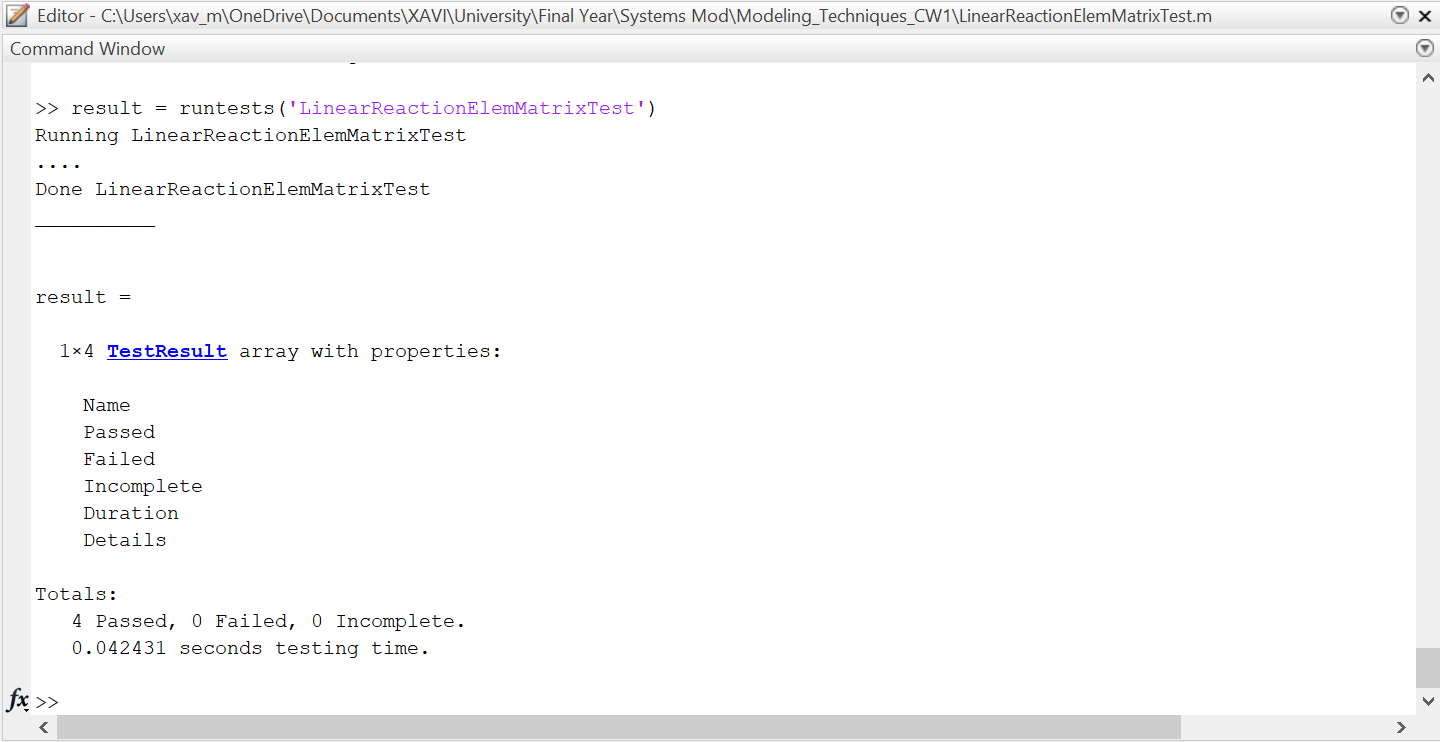
\includegraphics[width=0.9\textwidth]{LRtest2.PNG}
	\caption{Screenshot of LinearReationElemMatrix.m Function Passing Unit Tests}\label{fig:passTest2}
\end{figure}

\subsection{Question 1c}
\subsubsection{Solving Laplace With Dirichlet Boundaries}

The finite element solver StaticReactDiffSolver.m  was used to solve

\begin{equation}
\label{eq:Laplace}
\frac{\partial^2 c}{\partial x^2} = 0
\end{equation}

over the domain $x = 0$ to $x = 1$ with the Dirichlet boundary conditions:

\begin{subequations}\label{eq:LaplaceBCs}
\begin{align}
c = 2 \ \ at \ \ x = 0 \\
c = 0 \ \ at \ \ x  = 1
\end{align}
\end{subequations}

The analytical solution is given by equation \ref{eq:LaplaceAnalytical}.

\begin{equation}\label{eq:LaplaceAnalytical}
c = 2(1-x)
\end{equation}

The result of the analytical solution has been plotted in Figure \ref{fig:LaplaceFig1} with the FEM results overlaid. The FEM solution is very accurate here because linear approximations have been used as our basis functions and the analytical solution is also linear. This allowed good results even with a low resolution 4 element mesh.

\begin{figure}[h!] 
    \centering
    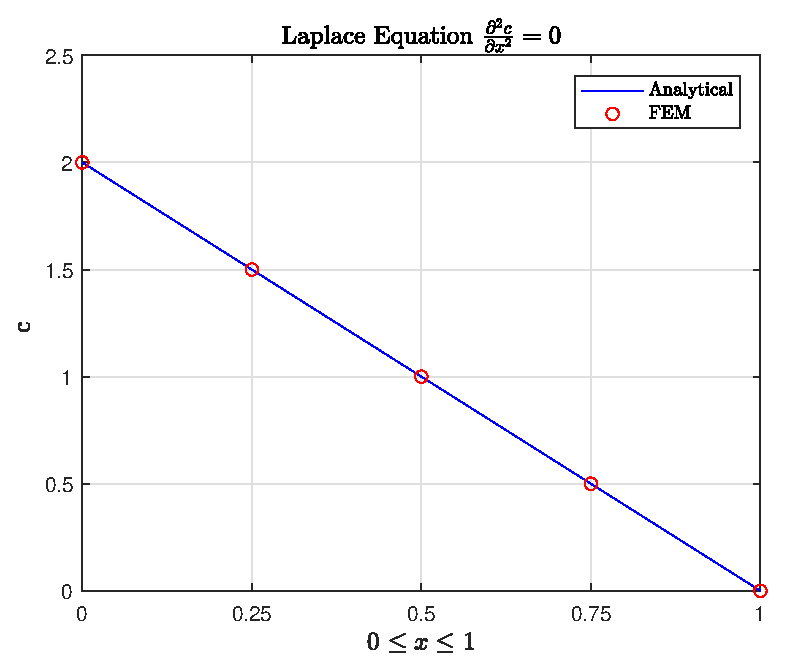
\includegraphics{epsLaplaceFig1}
    \caption{Comparison of Analytical and Finite Element Solutions of Laplace's Equation}\label{fig:LaplaceFig1}
\end{figure}

\subsubsection{Add a Neumann Boundary}
The initial boundary condition shall be changed to a Neumann boundary, the conditions are given by equations \ref{eq:LaplaceBCs21} and \ref{eq:LaplaceBCs22}.

\begin{subequations}
\begin{align}
\frac{dc}{dx} = 2 \ \ at \ \ x = 0 \label{eq:LaplaceBCs21} \\
c = 0 \ \ at \ \  x= 1 \label{eq:LaplaceBCs22}
\end{align}
\end{subequations}

\begin{figure}[h!] 
    \centering
    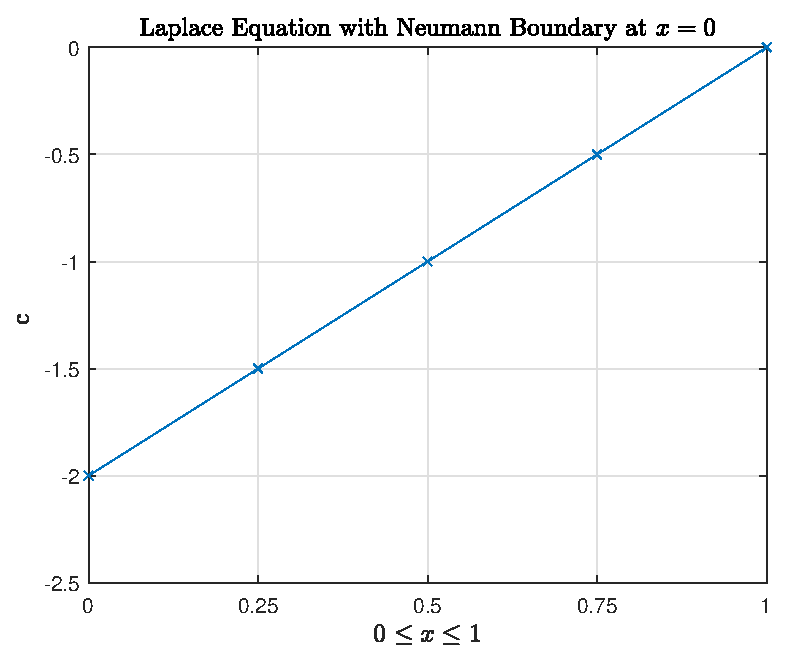
\includegraphics{epsLaplaceFig2}
    \caption{Using the FEM to solve Laplace's Equation with an initial Neumann Boundary}\label{fig:LaplaceFig2}
\end{figure}

The solution found using the FEM method with a 4 element mesh is plotted in Figure \ref{fig:LaplaceFig2}. The solution is still linear which is expected but the effect of change the initial boundary condition from $c = 2$ to $\frac{\partial c}{\partial x} = 2$ has meant $c = -2$ at $x = 0$. This is to be expected as the function is linear and therefore has a constant gradient over the domain which is defined by the Neumann condition. As the Dirichlet boundary is fixed at $c = 0$ at $x = 1$ in order to achieve the gradient $\frac{\partial c}{\partial x} = 2$ the only solution is $c = -2$ at $x = 0$. The same result could be achieved with a Dirichlet boundary of $c = -2$ at $x = 0$.

\subsection{Question 1d}

A reaction term will now be introduced to solve the static diffusion-reaction equation:

\begin{equation*}
D \frac{\partial^2 c}{\partial x^2} + \lambda c = 0
\end{equation*}

with the following parameters:

\begin{equation*}
D = 1, \ \  \lambda = -9
\end{equation*}

and the Dirichlet boundary conditions:


\begin{align*}
c = 0 \ \ at \ \ x = 0 \\
c = 1 \ \ at \ \  x= 1  .
\end{align*}


The analytical solution is given by equation \ref{eq:diffreactanalytical}. This has been plotted on Figure \ref{fig:ChangeMesh} along with the Finite Element Method solution for a range of mesh sizes. It can be seen how the FEM converges on the analytical solution as the mesh size is increased. For a mesh size of 3 elements there is a clear deviation from the analytical solution. This divergence is clearer towards $x = 1$ where the gradient of the analytical solution changes sharply and the linear approximation is least valid. However once the a mesh size is increased to 10 elements the plot is difficult to distinguish from the analytical solution and by 25 elements the error is less than 1\%.

\begin{equation}\label{eq:diffreactanalytical}
c(x) = \frac{e^3 }{e^6 - 1} (3e^{3x} - 3e^{-3x})
\end{equation}

\begin{figure}[ht] 

    \centering
    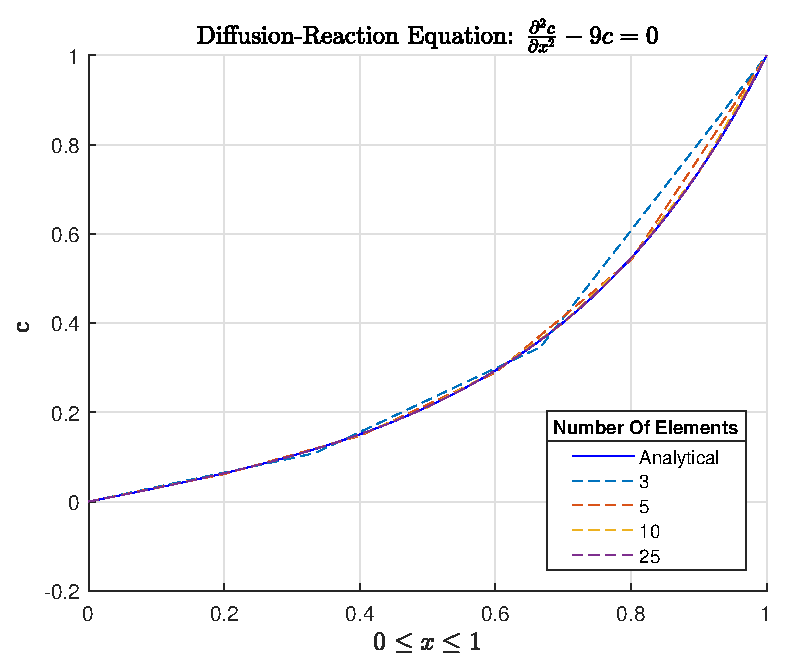
\includegraphics{epsReactDiff1}
    \caption{Using the FEM to solve the Static Diffusion-Reaction Equation with Dirichlet Boundary Conditions}\label{fig:ChangeMesh}
\end{figure}

\clearpage

%%%%\\\\\\\\\\\\\\\\\\\\\\\\\\\\\\\\PART 2 PART 2 PART 2///////////////////////////////////////////////////////////////%%%%%%%%%%%%%%%%%%%%%%%%

\section{Part 2}
\subsection{Question 2a}
\subsubsection{Setting The Equation}
The FEM method to find the temperature profile through a material filled with small diameter heating channels. The cross section of the material is shown in Figure \ref{fig:CrossSection} and approximates to a 1D heat transfer problem given by equation \ref{eq:part2analytical1}.

\begin{figure}[h!] 
    \centering
    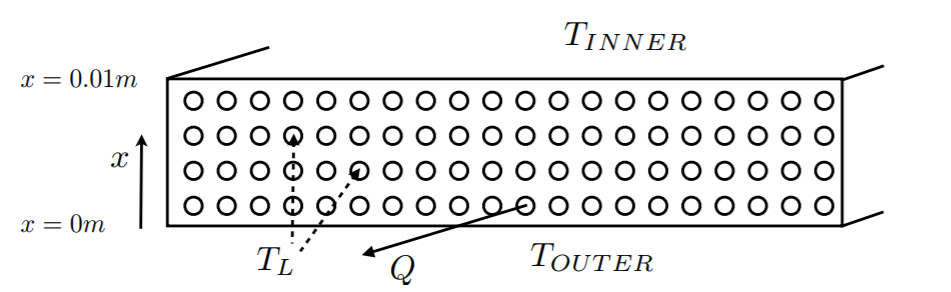
\includegraphics{CrossSection}
    \caption{Cross Section of Material.}\label{fig:CrossSection}
\end{figure}

\begin{equation} \label{eq:part2analytical1}
k \frac{\partial^2 T}{\partial x^2} + Q(T_L - T) = 0
\end{equation}

Rewriting this equation into the general diffusion-reaction equation form given by equation \ref{eq:MAIN} gives us \ref{eq:inDRgeneralform}.

\begin{subequations}
\begin{align}
D \frac{\partial^2c}{\partial x^2} + \lambda c + f = 0 \label{eq:DRgeneral} \\
D \frac{\partial^2T}{\partial x^2} + (-Q) T + QT_L = 0 \label{eq:inDRgeneralform}
\end{align}
\end{subequations}


The range of liquid flow rates, $Q$, and liquid temperatures, $T_L$ is given below.

\begin{align*}
&Q = 0.5 \ \text{to} \ 1.5  \\
&T_L = 294.15K \ \text{to}\ 322.15K \ \ 
\end{align*}
\clearpage
\subsubsection{Effect of Varying Liquid Flow Rate}
The equation was solved for a range of values of Q and the results plotted. This was repeated for four values of $T_L$ and the results are shown in Figure \ref{fig:varyQmulti}. 

\begin{figure*}[ht] 
        \centering
        \begin{subfigure}[b]{0.475\textwidth}
            \centering
            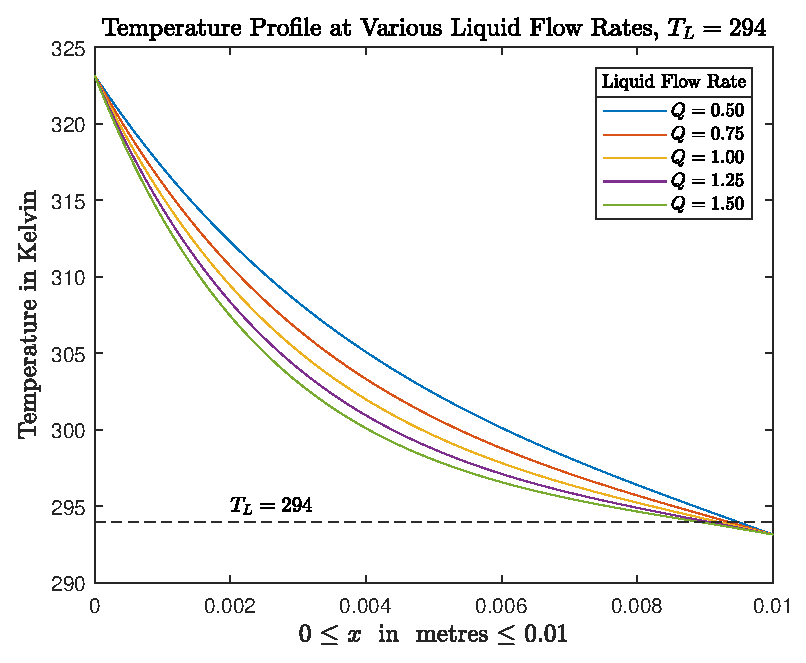
\includegraphics[width=\textwidth]{epsVaryQ294}
            \caption[Network2]%
            {{\small  }}    
            \label{fig:varyQ14}
        \end{subfigure}
        \hfill
        \begin{subfigure}[b]{0.475\textwidth}  
            \centering 
            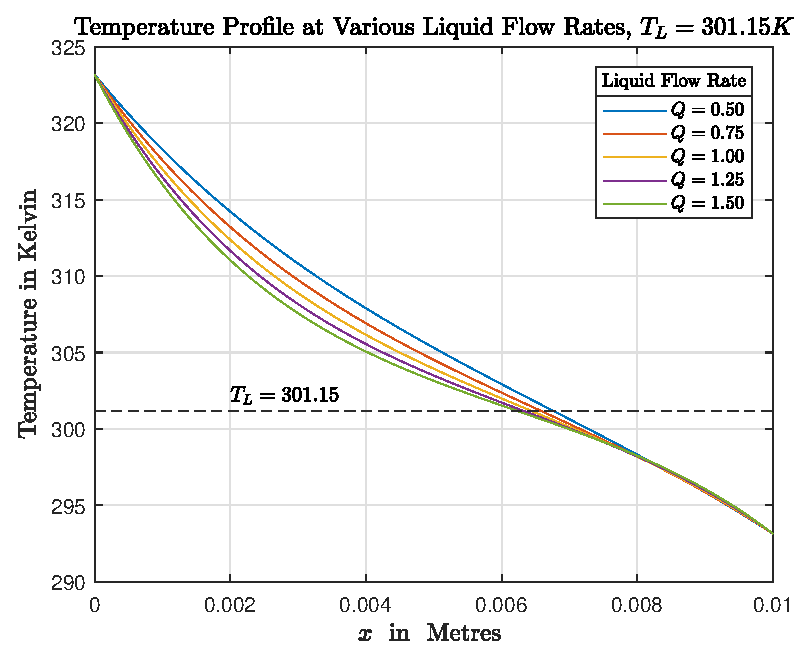
\includegraphics[width=\textwidth]{epsVaryQ301}
            \caption[]%
            {{\small }}    
            \label{fig:varyQ24}
        \end{subfigure}
        \vskip\baselineskip
        \begin{subfigure}[b]{0.475\textwidth}   
            \centering 
            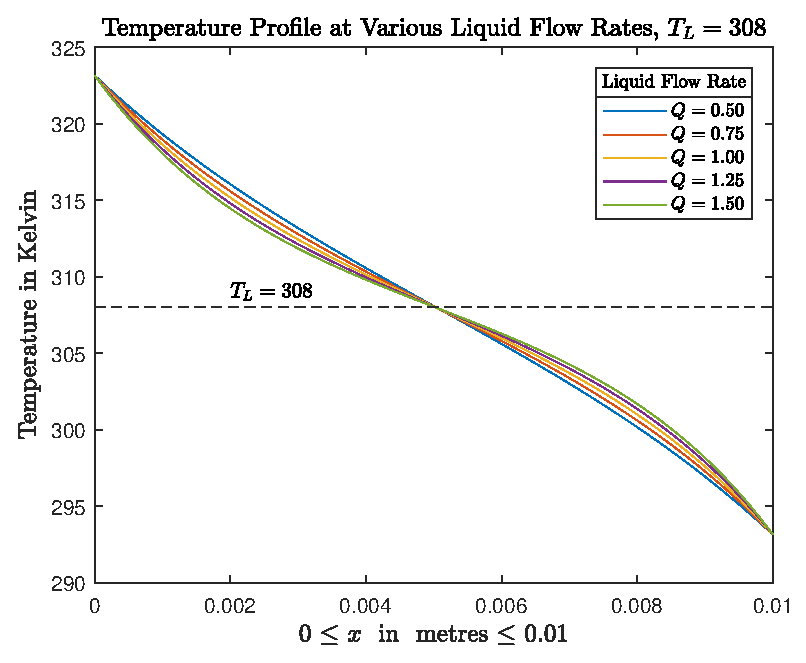
\includegraphics[width=\textwidth]{epsVaryQ308}
            \caption[]%
            {{\small }}    
            \label{fig:varyQ34}
        \end{subfigure}
        \quad
        \begin{subfigure}[b]{0.475\textwidth}   
            \centering 
            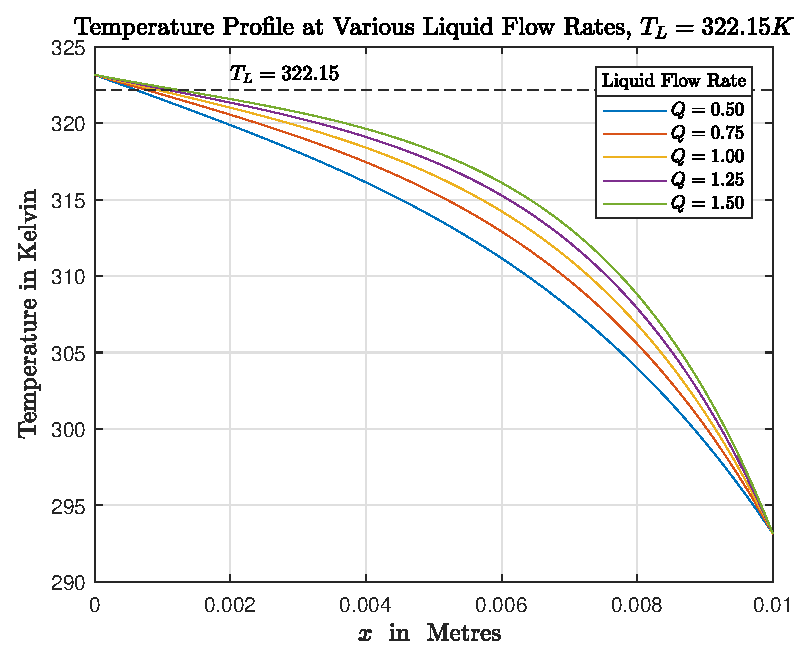
\includegraphics[width=\textwidth]{epsVaryQ322}
            \caption[]%
            {{\small }}    
            \label{fig:varyQ44}
        \end{subfigure}
        \caption[ The Effect of Varying the Liquid Flow Rate on Temperature Distribution and Gradient]
        {\small The Effect of Varying the Liquid Flow Rate on Temperature Distribution and Gradient} 
        \label{fig:varyQmulti}
    \end{figure*}

The effect of increasing the liquid flow rate is to bring the temperature profile towards the liquid temperature. This is most evident when their is a large differential temperature between the liquid and a boundary condition as a large temperature differential means a lot of heat can be transferred. For example in Figure \ref{fig:varyQ14} the liquid temperature is much cooler than the left hand boundary and so is heated by the material. As the thermal energy is transferred to the liquid its temperature rises reducing the differential temperature which reduces the rate of heat transfer. With higher flow rates the liquid temperature does not rise as much and so there is more heat transfer and steeper temperature gradient at and near the LHS boundary compared to the lower flows. 


\clearpage
\subsubsection{Effect of Varying Liquid Temperature}
\begin{figure*}[ht] 
        \centering
        \begin{subfigure}[b]{0.475\textwidth}
            \centering
            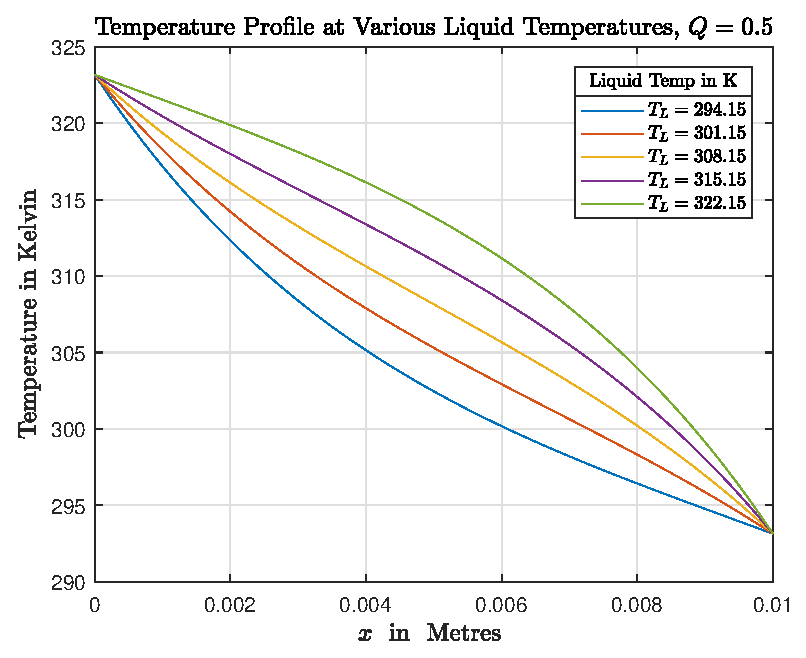
\includegraphics[width=\textwidth]{epsVaryTL1}
            \caption[Network2]%
            {{\small  }}    
            \label{fig:varyQ14}
        \end{subfigure}
        \hfill
        \begin{subfigure}[b]{0.475\textwidth}  
            \centering 
            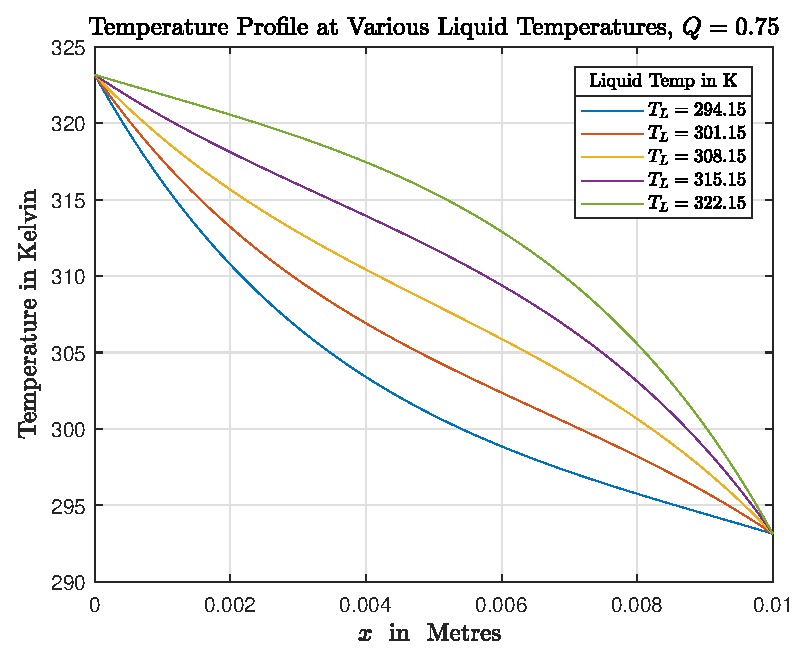
\includegraphics[width=\textwidth]{epsVaryTL2}
            \caption[]%
            {{\small }}    
            \label{fig:varyQ24}
        \end{subfigure}
        \vskip\baselineskip
        \begin{subfigure}[b]{0.475\textwidth}   
            \centering 
            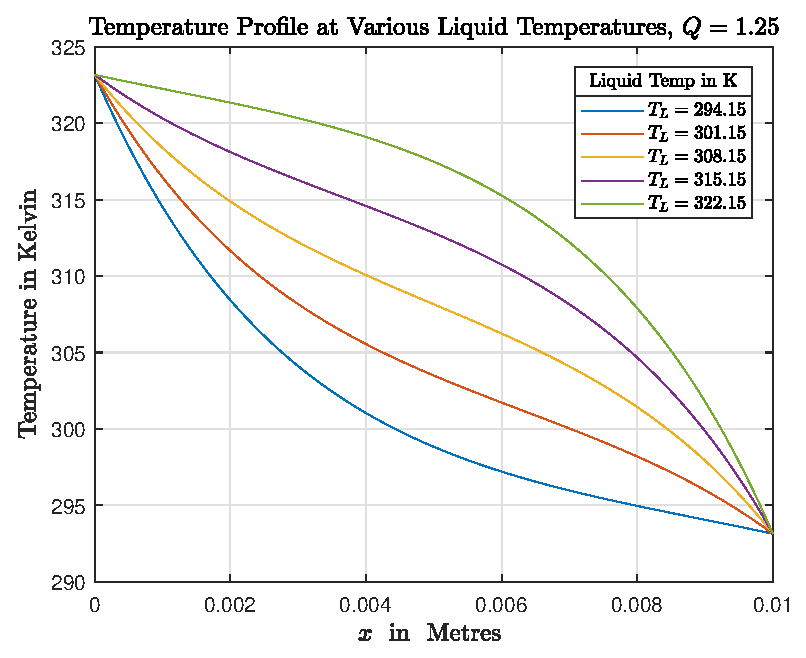
\includegraphics[width=\textwidth]{epsVaryTL4}
            \caption[]%
            {{\small }}    
            \label{fig:varyQ34}
        \end{subfigure}
        \quad
        \begin{subfigure}[b]{0.475\textwidth}   
            \centering 
            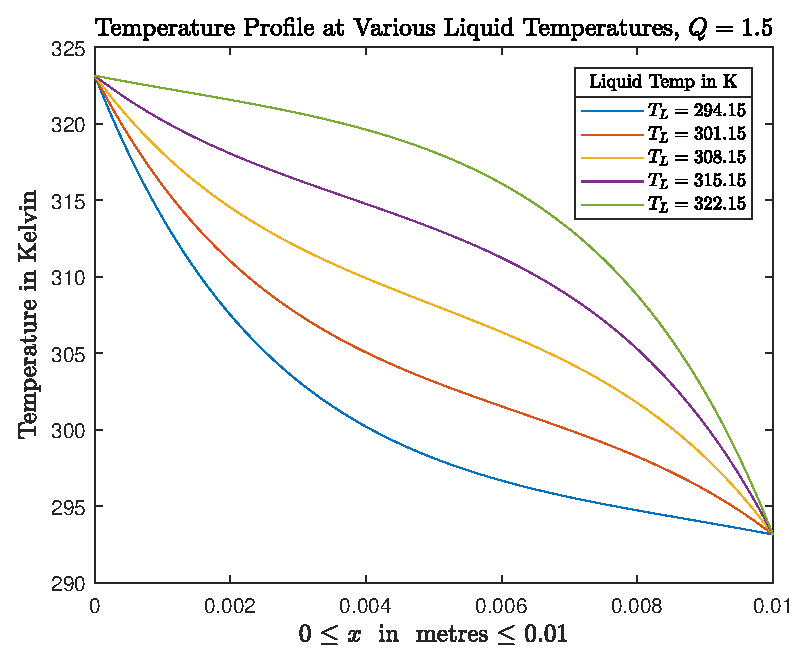
\includegraphics[width=\textwidth]{epsVaryTL5}
            \caption[]%
            {{\small }}    
            \label{fig:varyQ44}
        \end{subfigure}
        \caption[ The Effect of Varying the Liquid Temperature on Temperature Distribution and Gradient ]
        {\small The Effect of Varying the Liquid Temperature on Temperature Distribution and Gradient} 
        \label{fig:tempvar}
    \end{figure*}

Figure \ref{fig:tempvar} show how the liquid temperature determines the curvature of the temperature profile. When the liquid temperature is at 308.15k the temperature profile is relatively linear as this temperature is the mid-point between the two boundary conditions. When the liquid temperature increases the profile becomes more parabolic and convex. Similarly as the temperature decreases the profile becomes more parabolic and concave. Again this effect is more pronounced with higher liquid flows rates.

\clearpage

\subsubsection{Effect of Mesh Size}

To run the solver efficiently minimum mesh size which provides sufficient resolution is needed. To find the appropriate mesh size the least linear solution needs to be used which is the highest liquid flow rate $Q = 1.5$ and minimum liquid temperature $T_L = 294.15$. The solution for several mesh sizes is shown in Figure \ref{fig:fullviewmesh}. 

\begin{figure}[h!]
    \centering
    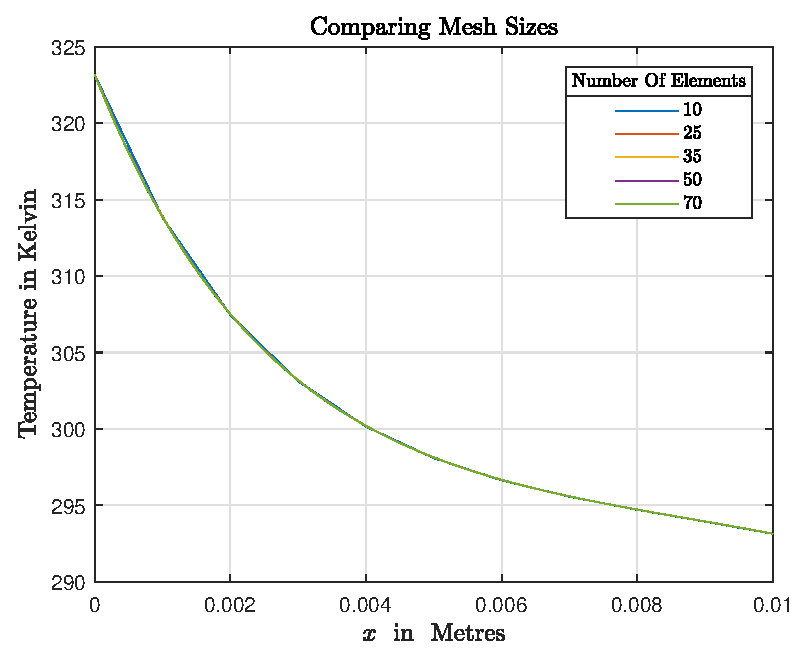
\includegraphics{epsMesh01}
    \caption{Cross Section of Material }\label{fig:fullviewmesh}
\end{figure}
\clearpage
\begin{figure*}[ht] 
        \centering
        \begin{subfigure}[b]{0.475\textwidth}
            \centering
            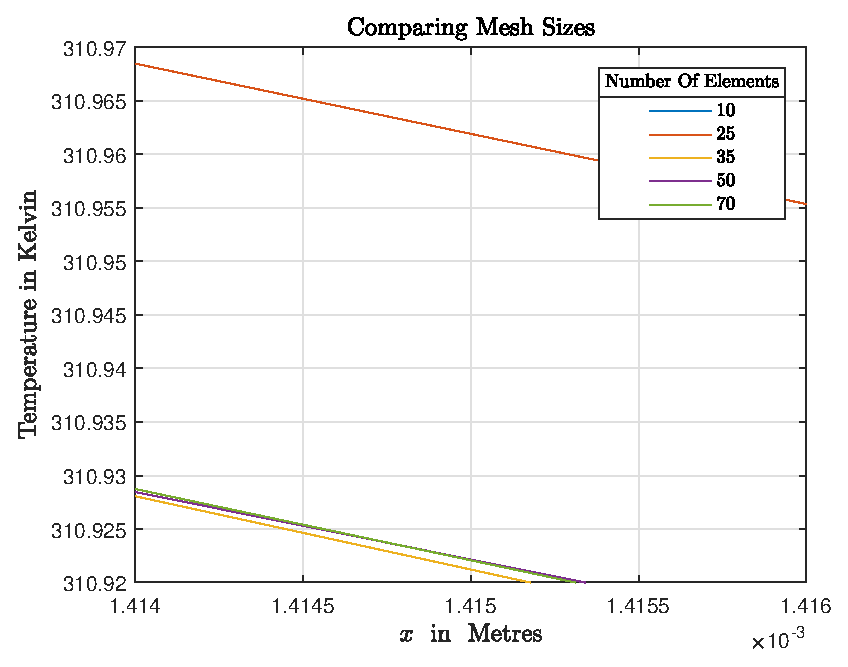
\includegraphics[width=\textwidth]{epsMesh11}
            \caption[Network2]%
            {{\small  }}    
            \label{fig:zoommesh1}
        \end{subfigure}
        \hfill
        \begin{subfigure}[b]{0.475\textwidth}  
            \centering 
            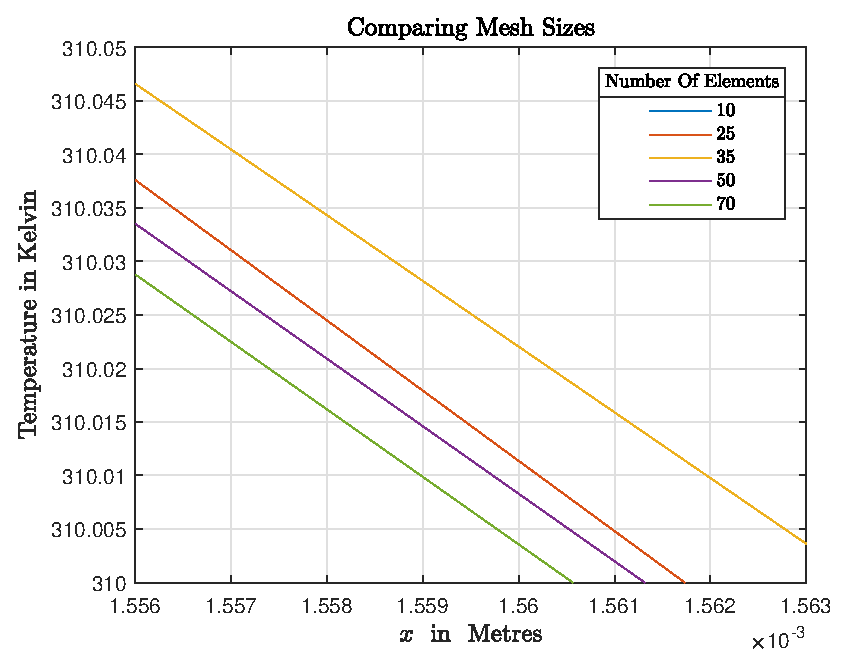
\includegraphics[width=\textwidth]{epsMesh12}
            \caption[]%
            {{\small }}    
            \label{fig:zoommesh2}
        \end{subfigure}
        \caption[ The Effect of Mesh Size on Temperature Resolution ]
        {\small The Effect of Mesh Size on Temperature Resolution} 
        \label{fig:meshzoom}
    \end{figure*}

An acceptable resolution for temperature is .01K as only very specialised and expensive temperature sensors have greater accuracy than this. In Figure \ref{fig:zoommesh1} it appears as though the 35, 50 and 70 element meshes have all converged to well within 0.01k. Figure \ref{fig:zoommesh2}, which is at the same temperature scale as Figure \ref{fig:zoommesh1}, shows that this convergence does not hold over the entire domain. The 35 element mesh is now approximately .02k above the 70 element mesh however the 50 and 70 element meshes are still within .01K. Figure \ref{fig:zoommesh2} is at one of the points in Figure \ref{fig:fullviewmesh} with the greatest divergence in solutions and so it can be said that a 70 element mesh is provides the required resolution.

\clearpage

\subsection{Question 2b}

\subsubsection{Derivation of Linear Source Term}

The temperature of the liquid is changed to be a function of $x$  resulting in a new governing equation described by equation \ref{eq:2bmain}.

\begin{equation} \label{eq:2bmain}
k \frac{\partial^2 T}{\partial x^2} + Q(T_L(1 + 4x) - T) = 0
\end{equation}



The equation can be rearranged to the standard form as given by equation \ref{eq:DRgeneral} which gives us equation \ref{eq:2bDRform}.
\begin{equation} \label{eq:2bDFform}
k \frac{\partial^2 T}{\partial x^2} + (-Q)T + \left [ QT_L + 4QT_Lx \right ] = 0
\end{equation}

This is the same as equation \ref{eq:inDRgeneralform} but with an extra source term $4QT_Lx$. To derive the source term vector the following integral from equation \ref{eq:MAIN} needs to be solved.

\begin{equation*}
\int_{0}^{1}vf dx = \int_{0}^{1}v\left [ QT_L + 4QT_Lx \right ] dx
\end{equation*}

This can be split into the sum of two separate integrals as follows.

\begin{equation*}
\int_{0}^{1}v\left [ QT_L + 4QT_Lx \right ] dx = \int_{0}^{1}v QT_L dx + 4QT_L\int_{0}^{1}vx dx
\end{equation*}

Split this integration into a sum of elements as shown below for four elements.

\begin{equation*}
\int_0^1 4QT_Lx dx = \int_0^\frac{1}{4} 4QT_Lx dx + \int_\frac{1}{4}^\frac{2}{4}4QT_Lx  dx + \int_\frac{2}{4}^\frac{3}{4}  4QT_Lx dx + \int_\frac{3}{4}^1 4QT_Lx dx
\end{equation*}


Applying the Jacobi to map to the $\zeta$ domain and taking constants out of the integral gives the following.

\begin{equation} \label{eq:LinSJ}
\int_{x_0}^{x_1} = 4QT_L\int_{-1}^1 vxJ d\zeta
\end{equation}

To solve this extra term it is necessary to use the basis function for $x$ given by equation \ref{eq:LagrangeX} and shown below as well as the basis function for $v$.

\begin{align*}
&x = x_{0}\psi_{0}(\zeta) + x_1\psi_{1}(\zeta) \\
&v = \psi_{0}, \psi_{1}
\end{align*}

As before this gives a set of two integrals which can be written in matrix form as shown below.


\begin{subequations}
\label{eq:linSsim}
\begin{align}
&4QT_LJ \left  [x_0 \int_{-1}^{1} \psi_{0} \psi_{0} d \zeta + x_1 \int_{-1}^{1} \psi_{1} \psi_{0} d\zeta ) \right ] \label{eq:linsrow1} \\
&4QT_LJ  \left  [x_0 \int_{-1}^{1} \psi_{0} \psi_{1} d \zeta + x_1 \int_{-1}^{1} \psi_{1} \psi_{1} d\zeta ) \right ]  \label{eq:linsrow2} 
\end{align}
\end{subequations}



\begin{equation} \label{eq:linSmatrix}
4QT_LJ 
\begin{bmatrix}

Int_{00} & Int_{01} \\
Int_{10} & Int_{11}
\end{bmatrix}
\begin{bmatrix}

x_{0} \\  x_{1} 
\end{bmatrix}
\end{equation}


We shall now evaluate the $Int_{nm}$ integrals to derive the matrix. It can be noted that these are the same $Int_{nm}$ terms that were solved to derive the reaction element matrix and so the same result should be found.

\underline{$Int_{00}$} \\
\begin{equation}\label{eq:LSInt00}
\begin{split}
 Int_{00} &= \int_{-1}^{1} \psi_{0}\psi_{0} \ d \zeta \\
&=  \int_{-1}^{1}  \Big ( \frac{1-\zeta}{2} \Big )^2 d\zeta \\
& = \left[ \frac{1}{3} \Big ( \frac{1-\zeta}{2} \Big )^3 (-2) \right]_{-1}^{1} \\
& = \frac{2}{3}
\end{split}
\end{equation}

\underline{$Int_{01} = Int_{10}$} \\

\begin{equation}\label{eq:LSInt01}
\begin{split}
 Int_{00} &= \int_{-1}^{1} \psi_{0}\psi_{1} \ d \zeta \\
&=  \int_{-1}^{1}  \Big ( \frac{1-\zeta}{2} \Big )  \Big ( \frac{1+\zeta}{2} \Big )d\zeta \\
& = \left[ \frac{\zeta}{4} - \frac{\zeta^3}{12}\right]_{-1}^{1} \\
& = \left[ \frac{1}{6} -  \Big (-\frac{1}{4} + \frac{1}{12} \Big )\right]_{-1}^{1} \\
& = \frac{1}{3}
\end{split}
\end{equation}

\underline{$Int_{11}$} \\
\begin{equation}\label{eq:LSInt00}
\begin{split}
 Int_{00} &= \int_{-1}^{1} \psi_{1}\psi_{1} \ d \zeta \\
&=  \int_{-1}^{1}  \Big ( \frac{1+\zeta}{2} \Big )^2 d\zeta \\
& = \left[ \frac{1}{3} \Big ( \frac{1+\zeta}{2}\Big)^3 . 2 \right]_{-1}^{1} \\
& = \frac{2}{3}
\end{split}
\end{equation}



Now putting substituting these results into the matrix form to get the following solution for the local element vector linear source terms, $f_L$ at the local element nodes 0 and 1. These local linear source nodes can be added to the local 'scalar' source nodes created for the $QT_L$ term, thus deriving the global source matrix needed for the FEM solver.


%%%LINEAR SOURCE MATRIX%%%%%%%
\begin{equation} \label{eq:linSresult}
\begin{bmatrix}
f_{L_0}\\[1ex]
 f_{L_1} 
\end{bmatrix}
= 4QT_L J 
\begin{bmatrix}
\frac{2}{3} & \frac{1}{3}  \\[1ex]
 \frac{1}{3}  & \frac{2}{3}
\end{bmatrix}
\begin{bmatrix}
x_{0} \\[1ex] x_{1} 
\end{bmatrix}
\end{equation}
\clearpage


\subsubsection{Linear Source Results}

\begin{figure*}[ht] 
        \centering
        \begin{subfigure}[b]{0.475\textwidth}
            \centering
            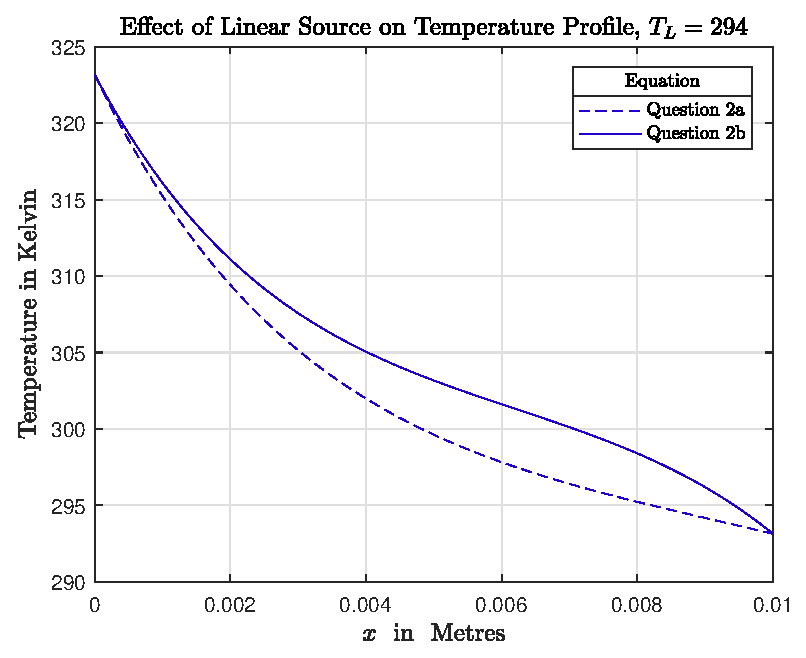
\includegraphics[width=\textwidth]{epsLinear294}
            \caption[Network2]%
            {{\small  }}    
            \label{fig:Linear294}
        \end{subfigure}
        \hfill
        \begin{subfigure}[b]{0.475\textwidth}  
            \centering 
            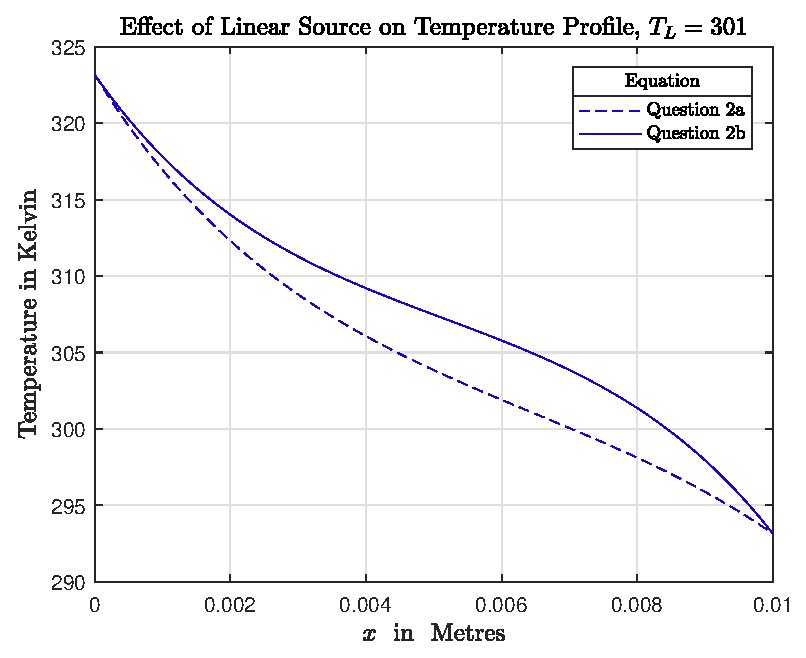
\includegraphics[width=\textwidth]{epsLinear301}
            \caption[]%
            {{\small }}    
            \label{fig:Linear301}
        \end{subfigure}
        \vskip\baselineskip
        \begin{subfigure}[b]{0.475\textwidth}   
            \centering 
            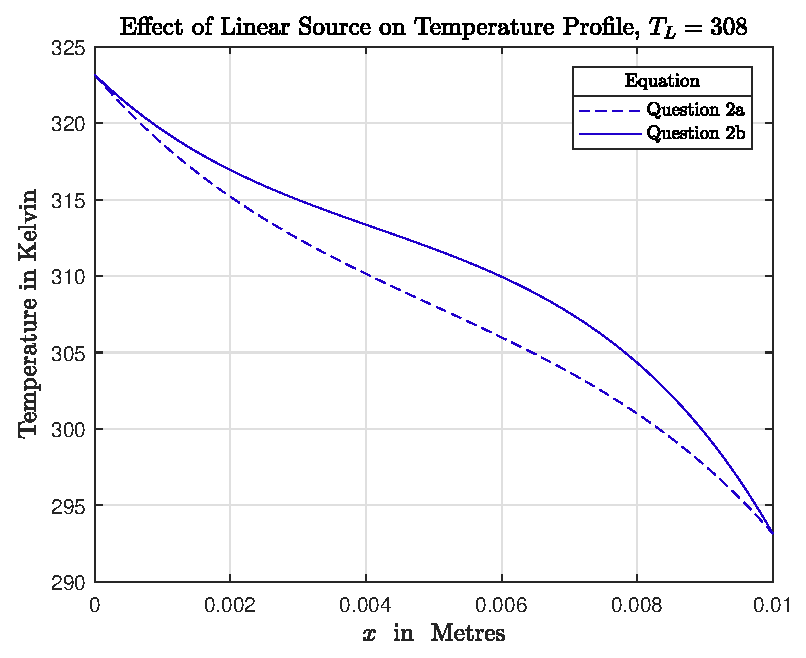
\includegraphics[width=\textwidth]{epsLinear308}
            \caption[]%
            {{\small }}    
            \label{fig:Linear308}
        \end{subfigure}
        \quad
        \begin{subfigure}[b]{0.475\textwidth}   
            \centering 
            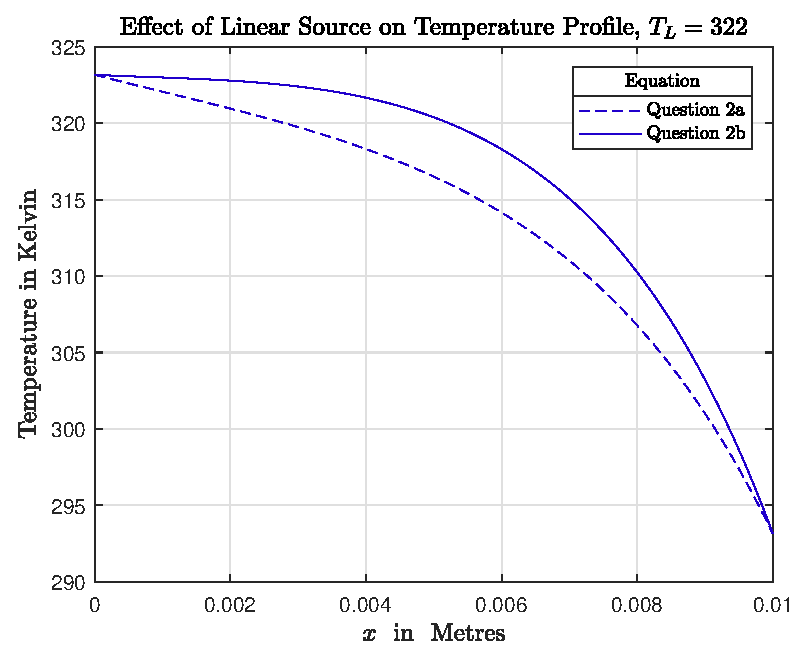
\includegraphics[width=\textwidth]{epsLinear322}
            \caption[]%
            {{\small }}    
            \label{fig:Linear322}
        \end{subfigure}
        \caption[ The Effect of Varying the Liquid Temperature on Temperature Distribution and Gradient ]
        {\small The Effect of Varying the Liquid Temperature on Temperature Distribution and Gradient ($Q =1$)} 
        \label{fig:LinearF}
    \end{figure*}

Figure \ref{fig:LinearF} shows how the linear source term, which represents the liquid temperature rising as $x$ increases, raises the temperature profile at the right hand boundary compared to the constant liquid temperature case.

%\begin{thebibliography}{9}
%%Last name, First Initial, Year published. Title. Publisher, Volume, Page(s).
%% HARVARD REFERENCE STYLE:
%%Brunner, F.H., 1949. Synthetic gasoline from natural gas. Industrial and engineering chemistry, 41(11), pp.2511-2515.
%
%\bibitem{SPEC} 
%Macgregor, K., 2017. 
%\textit{Student Design Project Specification 2017/18.}
%Airbus Group.


%\end{thebibliography}

\pagebreak

\begin{appendices}
%%AAAAAAAAAAAAAAAAAAAAAAAAAA%%%%%%%
\section{Laplace Element Matrix Code}\label{ap:LaplaceElem}
\begin{lstlisting}
function [SqMatrix] = LaplaceElemMatrix(D, eID, msh)

%Returns the local 2x2 element matrix of a given element for a given diffusion
%coefficient
%
% Inputs: 
% D - Coefficient of Diffusion
% eID - Index of element within mesh structure
% msh - Mesh which contains local elements within it's structure

%% Form of Laplace Elem matrix for J=1, D=1

SqMatrix = [0.5, -0.5; ...
            -0.5, 0.5];

%% Multiply  by (1/J) and D to get solution for the particular element

J = msh.elem(eID).J;  %Get Jacobi for the element

SqMatrix = (1/J) * D * SqMatrix;   %Local element matrix for element eID
end

\end{lstlisting}
\pagebreak

%%%%%%%%AAAAAA222222222A2A2AA22A2222222222AAAAAAAAA%%%%%
\section{CourseworkOneUnitTest.m}
\label{ap:CW1}
\begin{lstlisting}
%% Test 1: test symmetry of the matrix
% Test that this matrix is symmetric
tol = 1e-14;
D = 2; %diffusion coefficient
eID=1; %element ID
msh = OneDimLinearMeshGen(0,1,10);

elemat = LaplaceElemMatrix(D,eID,msh); %THIS IS THE FUNCTION YOU MUST WRITE

assert(abs(elemat(1,2) - elemat(2,1)) <= tol)

%% Test 2: test 2 different elements of the same size produce same matrix
% % Test that for two elements of an equispaced mesh, as described in the
% % lectures, the element matrices calculated are the same
tol = 1e-14;
D = 5; %diffusion coefficient
eID=1; %element ID
msh = OneDimLinearMeshGen(0,1,10);

elemat1 = LaplaceElemMatrix(D,eID,msh);%THIS IS THE FUNCTION YOU MUST WRITE

eID=2; %element ID

elemat2 = LaplaceElemMatrix(D,eID,msh);%THIS IS THE FUNCTION YOU MUST WRITE

diff = elemat1 - elemat2;
diffnorm = sum(sum(diff.*diff));
assert(abs(diffnorm) <= tol)

%% Test 3: test that one matrix is evaluted correctly
% % Test that element 1 of the three element mesh problem described in the lectures
% % the element matrix is evaluated correctly
tol = 1e-14;
D = 1; %diffusion coefficient
eID=1; %element ID
msh = OneDimLinearMeshGen(0,1,3);

elemat1 = LaplaceElemMatrix(D,eID,msh);%THIS IS THE FUNCTION YOU MUST WRITE

elemat2 = [ 3 -3; -3 3];
diff = elemat1 - elemat2; %calculate the difference between the two matrices
diffnorm = sum(sum(diff.*diff)); %calculates the total squared error between the matrices
assert(abs(diffnorm) <= tol)
\end{lstlisting}
\pagebreak


%%%%%%%%BBBBBBBBBBBBBBBBBBBBBB%%%%%%%%%%%%%%%%%
\section{Linear Reaction Element Matrix Code} \label{ap:React}
\begin{lstlisting}
function [SqMatrix] = LinearReactionElemMatrix(lambda, eID, msh)

%Returns a local 2x2 element matrix of a given element for a diffusion
%operator
% Inputs: 
% lambda - Scalar Coefficient of Diffusion
% eID - Index of element within mesh structure
% msh - Mesh which contains local elements within it's structure

%% Form of Linear Reaction local element matrix for J = 1 and lambda = 1
SqMatrix = [(2/3), (1/3); ...
            (1/3), (2/3)];

%% Multiply by J and lambda to get solution for the particular element

J = msh.elem(eID).J;  %Get Jacobi for the element

SqMatrix = J * lambda .* SqMatrix;   %Local Linear Reaction matrix for element eID
end
\end{lstlisting}
\pagebreak
%%%%%%%%CCCCCCCCCCCCCCCCCCCC%%%%%%%%%%%%%%%%%
\section{Linear Reaction Element Matrix Test} \label{ap:ReactTest}
\begin{lstlisting}
%%%THIS SCRIPT TESTS LinearReactionElemMatrix.m WORKS CORRECTLY

%% Test 1: test symmetry of the matrix
% Test that this matrix is symmetric
tol = 1e-14;
lambda = 2; %diffusion coefficient
eID=1; %element ID
msh = OneDimLinearMeshGen(0,1,10);  %generate mesh using given funciton

elemat = LinearReactionElemMatrix(lambda,eID,msh); %Calculate Linear Element Matrix

assert(abs(elemat(1,2) - elemat(2,1)) <= tol && abs(elemat(1,1) - elemat(2,2))  <= tol, ...
    'Local element matrix is not symmetric!')
%% Test 2: test 2 different elements of the same size produce same matrix
%Test that for two elements of an equispaced mesh, as described in the
%lectures, the element matrices calculated are the same
tol = 1e-14;
lambda = 5; %diffusion coefficient
eID=1; %element ID
msh = OneDimLinearMeshGen(0,1,10);

elemat1 = LinearReactionElemMatrix(lambda,eID,msh);	%calculate element 1 matrix

eID=2; %element ID

elemat2 = LinearReactionElemMatrix(lambda,eID,msh); %calculate element 2 matrix

diff = elemat1 - elemat2;
diffnorm = sum(sum(diff.*diff));
assert(abs(diffnorm) <= tol)

%% Test 3: test that one matrix is evaluted correctly
% % Test that element 1 of the three element mesh problem described 
% in Tutorial 3 Question 2c has the element matrix evaluated correctly
tol = 1e-14;
lambda = 1; %diffusion coefficient
eID=1; %element ID
msh = OneDimLinearMeshGen(0,1,6);

elemat1 = LinearReactionElemMatrix(lambda,eID,msh); %calculate element 1 matrix

elemat2 = [ (1/18), (1/36); (1/36), (1/18)];    % This is the known result
diff = elemat1 - elemat2; %calculate the difference between the two matrices
SummedDiff = sum(sum(diff)); %calculates the sum of the elements in the diff matrix
assert(abs(SummedDiff) <= tol) %Checks the error of the summed differences is below tol

%% Test 4: test main diagonal values are double antidiagonal values
% using random inputs for number of elemnts and lambda
tol = 1e-14;
lambda = 5*abs(rand(1,1)); %returns random diffusion coefficient between 0 and 4
eID=1; %element ID
ne = randi([4 100], 1,1);     %sets number of elements to random integer between 4 and 100
msh = OneDimLinearMeshGen(0,1,ne);

elemat1 = LinearReactionElemMatrix(lambda,eID,msh);
elem = elemat1(1,1)/elemat1(2,1); %Gets ratio between 1,1 and 2,1 elements
assert(abs(elem - 2) <= tol)     %Checks ratio is 2 within the tolerance
\end{lstlisting}
\pagebreak




%%%%%%%%DDDDDDDDDDDDDDD%%%%%%%%%%%%%
\section{Apply Boundary Condition Code} \label{ap:BC}
\begin{lstlisting}
function [GlobalMatrix, F] = ApplyBCs(BC, GlobalMatrix, F, ne)
% Applies boundary conditions to F and Global Matrix as appropriate
% for the specified boundary condition
%
%Inputs:
%BC - Structure which contains the following:
%       BC(1) - Holds data for minimum x boundary
%       BC(2) - Holds data for maximum x boundary
%       BC().type - Type of boundary condition: "neumann", "dirichlet" or
%                   "none" (must be a lower case string)
%       BC().value - Value of the boundary condition (float or int)
%
%GlobalMatrix - formation of local element matrices (NxN matrix)
%F - Source Vector (size Nx1 vector)

%% Solve xmin Boundary Condition 
if BC(1).type == "none" %No action needed if no boundary condition
    % pass 
    
elseif BC(1).type == "dirichlet"  %solve for a dirichlet BC
    
    %set all first row elements to 0 except first element  
    GlobalMatrix(1,:) = [1, zeros(1,ne)];   
    %set first element of the source vector to the xmin BC value
    F(1) = BC(1).value;
    
elseif  BC(1).type == "nuemann"    %solve for a nuemann BC
    
    %subtract the xmin BC value from the first element of the source vector 
    F(1) = F(1) - BC(1).value;
end

%% Solve xmax Boundary Condition
if BC(2).type == "none" %No action needed if no boundary condition
    % pass
    
elseif BC(2).type == "dirichlet"  %solve for dirichlet BC
    
    %set all first row elements to 0 except last element 
    GlobalMatrix(end,:) = [zeros(1,ne), 1];
    %set last element of the source vector to the xmax BC value
    F(end) = BC(2).value;
    
elseif BC(2).type == "nuemann"    %solve nuemann BC
    
    %subtract the xmin BC value from the last element of the source vector 
    F(end) = F(end) + BC(2).value;
end   
end

\end{lstlisting}
\pagebreak



%%%%%%%%EEEEEEEEEEEEEEEEEEEEEEEEEEEE%%%%%%%%%%%%%
\section{Static Diffusion-Reaction Solver Code}
\label{ap:SDRS}
\begin{lstlisting}
function [mesh] = StaticReactDiffSolver(lambda, D, xmin, xmax, ne,f_scalar, f_linear,  BC)
%%% Solves the static reaction diffusion equation
% Inputs:
% lambda - Coefficient for Reaction (float ot int)
% D - Coefficient of Diffusion (float or int)
% xmin - Minimum value for x, usually 0(float or int)
% xmax - Maximum value for x, usually 1(float or int)
% ne - Number of Elements in Mesh (float)
% f_scalar - Constant Source Term (float or int)
% f_linear - Linear Source Term (float or int)
%BC - Structure which contains the following:
%       BC(1) - Holds data for minimum x boundary
%       BC(2) - Holds data for maximum x boundary
%       BC().type - Type of boundary condition: "neumann", "dirichlet" or
%                   "none" (must be a lower case string)
%       BC().value - Value of the boundary condition (float or int)

mesh = OneDimLinearMeshGen(xmin, xmax, ne); %Generate Mesh

GlobalMatrix = zeros((ne+1),(ne+1));  %Initiate Global Matrix

%% Generate the source the vector
F = SourceVectorGen(mesh, f_scalar, f_linear);

%% Assemble local element matrices into global matrix
for eID = 1:ne
    
    %Calculate Local Element Matrix for Diffusion Term
    DiffusionLocal = LaplaceElemMatrix(D, eID, mesh);
    
    %Calculate Local Element Matrix for Linear Reaction Term
    ReactionLocal = LinearReactionElemMatrix(lambda, eID, mesh);
    
    %Local Element Matrix is the Diffusion subtract the Linear Reation
    LocalElementMatrix = DiffusionLocal - ReactionLocal;
                        
    %Add Local Element Matrix into the correct location within the Global Matrix
    GlobalMatrix(eID:(eID+1),eID:(eID+1)) = GlobalMatrix(eID:(eID+1),eID:(eID+1))...
                                            + LocalElementMatrix;
end

%Apply Boundary Conditions
[GlobalMatrix, F] = ApplyBCs(BC, GlobalMatrix, F, ne);

%% Solve for C
C = GlobalMatrix \ F;

%Add values of C into the mesh structure
for i = 1:length(C)
    mesh.c(i) = C(i);
end

end
\end{lstlisting}
\pagebreak

%%%%%%%%FFFFFFFFFFFFFFFFFFFFFFFFFFFFFFFFF%%%%%%%%%%%%%
\section{Source Vector Generator} \label{ap:SVG}
\begin{lstlisting}
function [F] = SourceVectorGen(mesh, f_scalar, f_linear)
%Generates source vector
%Inputs:
%mesh - Mesh contains local elements and other data in it's structure
%f_scalar - Constant source term
%f_linear - Linear source term

ne = mesh.ne;   %Number of elements
J = mesh.elem(1).J; %Jacobi (assumed equally spaced mesh)

%% Initalise Scalar Part of Source Vector F and add in Scalar Part
F = ones((ne+1),1);
F = (2*f_scalar*J) .* F;
F(1) = f_scalar*J;
F(end) = f_scalar*J;

%% Add in the Linear Element Matrices
for eID = 1:ne
    %Caluculat Linear Source Local Element Matrix
    LinearSourceLocal = LinearSourceElemMatrix(mesh, eID, f_linear);
    %AddLocal Linear Source into Source Vector at correct location
    F(eID:(eID+1)) = F(eID:(eID+1)) + LinearSourceLocal;
end
\end{lstlisting}
\clearpage


%%%%%%%%%%%%GGGGGGGGGGGGGGGGGGGGGGGGGG%%%%%%%%%%%%%%%%%%

\section{Linear Source Vector} \label{ap:LSV}
\begin{lstlisting}
function [ElemVector] = LinearSourceElemVector(mesh, eID, f_linear)
% Returns the Local Linear Source Vector for an element
%
% Inputs:
% mesh - Mesh which contains local elements within it's structure and
%           related variables
% eID - index for the element within the mesh
% f_linear - Linear source term multiplier

%% Extract element variables from mesh
J =mesh.elem(1).J;      %Get Jacobi for the element
x0 = mesh.elem(eID).x(1);   %Get he x0 value for the element
x1 = mesh.elem(eID).x(2);   %Get he x1 value for the element
xVector = [x0;x1];          %Create a vector of the x values

%% Local Source Vector with J =1 and f_linear = 1
StandardVector = [(2/3), (1/3);...
                  (1/3), (2/3)];
              
%% Multiply by J, f_linear and the x vector to get Local Linear Source 
%Vector for the specific element
ElemVector = J * f_linear *  StandardVector * xVector;
end
\end{lstlisting}
\end{appendices}





\end{document}

